\documentclass[../main.tex]{subfiles}
\graphicspath{{\subfix{../images/}}}

\begin{document}
	
\chapter{Methodology}
\section{Introduction}


\todo{rewrite introduction}

To analyze the performance of different support structures created using topology optimization, a comparison study was made in which parts created by additive manufacturing were paired with different support structures. This study assumed that different structures will conduct heat energy differently, and thus some topologies might be more effective in removing heat faster from each material layer as it is being processed. This increased thermal conduction would then result in less overall thermal deformation, as the manufactured component would expand less due to the decreased time in high temperatures. 

This section will explain the full process taken to run the simulations and analyze the data. An overview of the process can be seen in Figure~\ref{fig:process_diagram}. The process starts from the creation of the CAD for the manufactured components, followed by the design and CAD creation of the support structures. The components and the support structures are then merged, and imported into the additive manufacturing software to simulate the results of manufacture. The results from the manufacturing simulation are then analyzed by means of graphs and statistical methods. 

\todo{Fix this process diagram}
\begin{figure}
  \begin{center}
    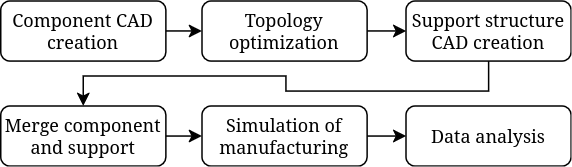
\includegraphics[width=0.95\textwidth]{process_diagram.png}
  \end{center}
  \caption{Process diagram.}\label{fig:process_diagram}
\end{figure}

The subsequent sections explain in detail each stage of this process.

\section{Component CAD creation}

\subsection{Simple geometry}

The components with simple geometries utilized in this study consist of a cube, three triangular
components with different slopes, and three cylindrical components with different values of
curvature. These shapes with these dimenions were chosen to ease the comparison of results between this study and the study of Peishu \cite{chungpei-hsuStudyLatticeSupport2024}. All the CAD models
used for the simple geometry study were created using FreeCAD, an open-source CAD software. The components were exported as .STEP files, and then were merged with their corresponding support structures using the software nTop. The geometries used for this preliminary study are the following:

\begin{itemize}
  \item A cube with side length of 30 mm (Figure \ref{fig:cube}).
  \item Three triangular components with varying slopes. All triangular components have a base of 30 x 30 $mm^2$, with slopes of 15 \degree, 30  \degree and 45 \degree. The measurements are shown in figure. \missingfigure{measurements of triangles.}
  \item Three prisms with rounded edge of different radii. The radii used were 20mm, 30mm, and 40mm. These rounded prisms also have a base of 30 x 30 $cm^2$. \missingfigure{pictures of cylinders}
\end{itemize}

\begin{figure}
	\begin{center}
		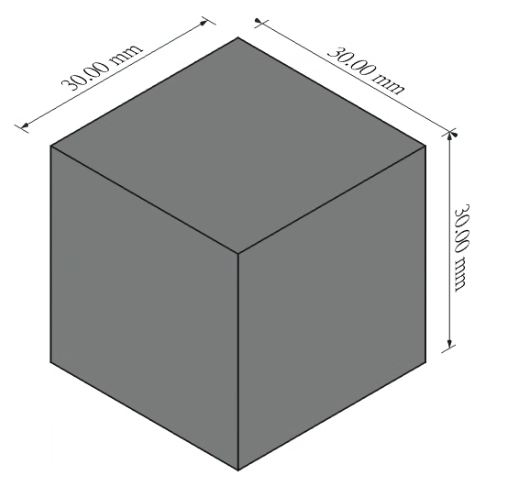
\includegraphics[width=0.45\textwidth]{cube.png}
	\end{center}
	\caption{Dimensions of cube component.}\label{fig:cube}
\end{figure}

\todo{Explain that design of femoral components is already done and is proprietary.}

\section{Topology optimization model}

The supporting structures of the components were created using the method of topology optimization. The design was implemented using the topology optimization module of COMSOL Multiphysics 6.2.  

The steps for creating a valid topology optimization model are: determine the design volume, design the support structure using topology optimization, merge the support structure with the part, and carry out the FEM simulation for manufacture.

\subsection{Design domain}

The design domain consisted of the volume between the bottom face of each component and the xy plane, when the component is placed at a height of 30mm above the xy plane. For the simple geometry parts, as they have high symmetry, the design domain was just taken to be a 2D slice of the volume. The topology optimization problem was then solved for this volume, and the resulting topologies were extruded in the direction perpendicular to the design plane to cover the space underneath the part. For the femoral component, the topology optimization was directly solved in the 3D volume between the lower surface of the femoral component and the xy plane.  

\subsection{Design of support structure using topology optimization}

The supporting structures were designed utilizing a SIMP topology optimization model with hyperbolic tangent filter. The mathematical model has been shown in equations \ref{eq:multiobj} - \ref{eq:vol}. The objective of the problem is to maximize the thermal conduction of the support structure, while at the same time maximizing its stiffness. The thermal conductivity has been chosen as an objective since it is required to drive heat away from the part as fast as possible to reduce its thermal deformation. 
Thermal conduction is given by Fourier's law as:

\begin{equation}
  \label{eq:Fourier Law}
  q = -k \nabla T
\end{equation}

where q is the heat conduction through the material, k is the material's thermal conductivity and $\nabla T$ is the thermal gradient. For use in a finite element solver, the above equation can also be written as:

\todo{thermal compliance equation goes here}.

At the same time, stiffness needs to be maximized to ensure that the supporting structure itself will not deform considerably. This might be caused by supporting structures made of very thin segments, which might buckle under the component's weight. In a worst case scenario, the structure itself would collapse, causing the whole manufacturing process to fail. In light of this, stiffness was also added as an objective. Stiffness, or compliance, can be written as:

\todo{equation for compliance here.},

where \todo{symbols of compliance}.

We can therefore combine these two together to obtain the objective function for the topology optimization problem:

\todo{Sum of objectives here}.

For this problem, the only restriction imposed on the system is a volume fraction constraint.

\subsection{Topology optimization equations}

\todo{Write the equqations here again. Remove reference of equation in previous paragraph.}
need to do this.

\section{COMSOL implementation}

\subsection{Mesh}

To run the topology optimization algorithm and obtain a solution, the design domain must be divided into finite element methods for computation. For the 2D design domains of the simple geometry elements, free triangular meshes were utilized, using a predefined mesh element size of "finer". This resulted in about 2000-3000 elements for each of the design domains, depending on the geometry of the domain. These mesh parameters were chosen to produce fast results and to obtain a general idea of how the simulation parameteres affected the solution of the topology optimization problem.

\missingfigure{Mesh of 2d design domain}

On the other hand, For the 3D design domain of the femoral component support structure, the mesh sizing parameters were chosen with more deliberation. The maximum and minimum element sizes of the mesh were determined based on the minimum element size achievable by the selective laser melting (SLM) machine utilized in this study, which is approximately 0.2 millimeters. However, employing a mesh with an element size of 0.2 millimeters results in excessively fine meshes that significantly prolong computational solving times. Consequently, the maximum and minimum mesh sizes were adjusted to be 8 and 4 times the minimum feature size, resulting in values of approximately 1.6 millimeters and 0.8 millimeters, respectively. This resulted in meshes with approximately 164,000 elements.

\missingfigure{Mesh of fem component support structure}


\subsection{Physical parameters}

\todo{Do this part}

For the topology optimization solution to be useful, realistic thermal and stress load should be used. The thermal load was based on the maximum wattage and efficiency of the laser achievable by the selective laser melting machine used in this work. The laser's power is 200W, with an efficiency of 25\%. This value cannot be used for the thermal load, since the laser is only activated for a small amount of time. From the FEM software building process parameters, each layer is heated for approximately 154 ms. Therefore, with an effective power of 200W x 0.25 = 50W, the total amount of energy added to the layer during the heating time is 50W x 154ms = 7.7 J. But each layer heating time occurs periodically, with a period of approximately 440s. Therefore, the average power input to the system per cycle is calculated to be 0.0175W. The approximate area of the top surface of the support structure design domain is approximately 30mm x 30mm = 900mm2. Diving the power per cycle by this area yields a heat flux of about 19.4 W/mm2, which was rounded up to 20.0 W/m2 for the topology optimization problem. For the heat flux used in the femoral component calculation, the difference is in the area of the top surface of the design domain. This area is about 1690 mm2, and thus the heat flux used for the support structure design in accounts to be about 10.37 W/m2, which was rounded to 10 W/m2.

\todo{Add material information here}
Need to talk about the material properties

\todo{Correct equations and figures in the above paragraph.}

\missingfigure{Graph of power heat cycle}

For the calculation of compliance, the structural load was also calculated by using the weight of each component and dividing it by the top area of the design domain. All of the components were modeled using the density of 316L steel, which is approximately 7.93 g / cm3. This was then multiplied by the volume of each component to obtain the mass. For example, the. The volume of the femoral component was calculated to be about 32800 mm3, and therefore the mass of the femoral component amounted to 0.263 kg. This was then divided by the top area of the design domain. Taking again the example of the femoral component's support structure, the area of the top surface is about 1690mm2, and so the average stress value of the top surface is calculated as 0.263 kg * g / 1690 mm2 = 1560 N/m2, where g is the gravitational constant. 

\subsection{Parametric study}

The topology optimization problem was solved using COMSOL Multiphysics 6.2 software. COMSOL allows the creation of parametric studies that allow to run a simulation with a list of parameters to be varied, in order to study the influence of different values on the solution of a system. For this study, the values of volume fraction, objective function weights, and hyperbolic tangent angle were chosen as the parameters to be varied.

Volume fraction is defined as the maximum amount of volume that the topology can cover within the design domain. This criteria is chosen because we seek to use less material for the supporting structure, as long as we can maintain the total deformation of the manufacturing componont beneath a threshold. For the simple geometries 50\% and 75\% of volume fraction were considered. For the femoral component study, volume fractions of 25\%, 33\%, 40\%, 50\% and 75\% were considered. 

The objective functions weights were also varied for the design of topologies for the simple geometry parts. \todo{Finish objective function weight explanation}

Finally, the hyperbolic tangent angle projection was also varied. \todo{Explain what the effect of hyp tan is and why the values were used. Explain that after theta = 8, all subsequejt values are the same, so this was the upper limit used.}

The values used in the parametric study are shown in tables \todo{add table reference here}.

\todo{Add tables of parameters here}

\subsection{Boundary conditions}

Explain that two boundary conditions were used for simple geometry, void and no void boundary.


\missingfigure{examples of comsol simulation}

\section{Creation of support structure CAD and merging with part}

After COMSOL was used to generate the possible topologies for the support structure, the topology was exported to image files, in the case of the 2D problem, and to an .STL file, in the case of the 3D structure. These were then converted to 3D .stp file with the aid of FreeCAD. nTop Software was then used to merge the resulting support structure with the manufactured components. Once the support structure and the part were joined, they were exported as .stl files to be used in the SLM finite element simulation.

Once the CAD file of the component and the support structure has been built, it is necessary to merge them together and import them into Simufact to undergo simulation of the manufacturing process. The software used for blending the component and its support structure is nTop \todo{add version here}. nTop's interface makes it very easy to merge the part, and also allows to blend the support structure and the component, which effectively creates a fillet between the nodes of both components to allow for a smooth transition between bodies. Of course, blending the component and the support structure in this manner would not give any benefit in a real manufacturing process, as the structure and the component would not be able to be separated easily. NEvertheless, this blend radius is beneficial for the simulation since it was observed that a direct union and import of the support structure + component in Simufact resulted in having very small gaps between the two pieces, resulting in a non manifold geometry that would cause the finite element model to have gaps between some of its nodes. 

\missingfigure{Figures of support structures with parts}

\section{Simulation of manufacturing process}

The software utilized to simulate the manufacturing process is Simufact Additive version 2023.2. Simufact Additive is capable of simulation building process of additive manufacturing components, and coupling thermal and stress physics to predict the temperature values of the component throughout the building process and the total stresses, strains and deformations resulting from the manufacturing process. 

In order to set up Simufact correctly, the building process and the building space geometry must be specified before each simulation. The building parameters and building geometries used in this study are the same that were used in the analysis of thermal deformation using lattice support structures done by Peihsy and al. \todo{add reference here}

\missingfigure{Need simulation process here: process properites -> build -> part import -> voxelization -> numerical parameters }

\subsection{Process properties}

\todo{add that thermomechanical process was used and explain what it is.}

After the component and the support structures were merged, they were imported into Simufact. It is during this step that all the factors related to the simulation are set, which include the machine properties, material properties, and build parameters. As mentioned previously, these were chosen to be identical to the study of PeiHsu to ensure that the results of this study could be compared to the results of that one. 

The first parameter to be chosen is the process properties, which determines the physics that Simufact takes into consideration to run the simulation. Simufact provides three different types of processes: mechanical, thermal, and thermomechanical. As stated in the Simufact manual \todo{insert reference to manual here}, mechanical provides a fast mechanical analysis that only uses inherent strains as the main input. This type of analysis does not take into consideration the temperature fields during the building process. The thermal process on the other hand only considers the thermal behaviour of the components, and the temperature field of the support structures, components and base can be analyzed. The thermomechanical process couples the stress and thermal analyses, and allows for the prediction of temperature, distortions and stresses of the part. This latter process is the one used in this study.

\subsection{Machine and build parameters}

After choosing the process property, the machine parameters must be specified. This includes the machine build plate geometry and the laser parameters. The machine build plate chosen was a circular plate with an 80 mm radius. The build space dimensions consists of a space of 160 mm in all three x-y-z directions. As for the laser parameters, the simulations were carried out with one laser with a maximum laser power of 500 W and a maximum laser speed of 2000 mm / s, an efficiency of 25 percent, and a beam width of 25 mm. All of these parameters are summarized in the table \todo{add the table of building parameters here.}

The building parameters for the process need also to be set. These include material layer parameters and any thermal parameters and temperature specifications for the build environment and base plate. The powder layer thickness was chosen to be 0.03 mm, with a recoater time of 10 s. The powder initial temperature was set to 25 \degree Celcius, with an initial base temperature of 200 degrees. \todo{explain why base plate temeprature might be used in practice, might want to add reference to 10.3390/thermo4010005}

\todo{Need to add exposure time, exposure energy fraction, and volumetric expansion factors here. Need to refer to Comsol documentation to explain what these are and how they influence the results.}

\todo{Need to say that no calibration was done. Explain why calibration is necessary for the manufacture of parts, but also explain the reason no calibration was done here.}

\todo{Explain what this is and how it is done, and what the purpose of this is.}

\begin{table}
  \centering
  \begin{tabular}{ |c|c| }
    \hline
    laser power & 200W \\
    \hline
    laser speed & 1000 mm/s \\
    \hline
    efficiency & 25\% \\
    \hline
    beam width & 100 $\mu$m \\
    \hline
    layer thickness & 30 $\mu$m \\
    \hline
    recoater time & 10 s \\
    \hline
  \end{tabular}
  \caption{Laser parameters}
  \label{tab:laser_params}
\end{table}

\begin{table}
  \centering
  \begin{tabular}{ |c|c| }
    \hline
    scan width & 20 mm \\
    \hline
    scan overlap & 0 mm \\
    \hline
    hatch distance & 0.07 mm \\
    \hline
    pause time & 0 s \\
    \hline
  \end{tabular}
  \caption{Scanner parameters}
  \label{tab:scanner_params}
\end{table}

\begin{table}
  \centering
  \begin{tabular}{ |c|c| }
    \hline
    powder temperature & 25 \degree C \\
    \hline
    chamber temperature & 50 \degree C \\
    \hline
    base plate temperature & 200 \degree C \\
    \hline
  \end{tabular}
  \caption{Thermal parameters}
  \label{tab:thermal_params}
\end{table}

\begin{table}
  \centering
  \begin{tabular}{ |c|c| }
    \hline
    Part / Support emissivity & 0.85 \\
    \hline
    Part / Support heat transfer coefficient & 12.0 $W/(m^2 K)$ \\
    \hline
    Base plate emissivity & 0.6 \\
    \hline
    Base plate heat transfer coefficient & 20 $W/(m^2 K)$ \\
    \hline
    Base plate contact heat transfer coefficient & 100 $W/(m^2 K)$\\
    \hline
  \end{tabular}
  \caption{Advanced thermal parameters}
  \label{tab:adv_thermal_params}
\end{table}

\subsection{Convergence analysis}

To ensure that FEM results were not dependent on the voxel size of the voxel mesh, a convergence analysis was first performed on one of the simple geometries. For this analysis, the results of three projects were compared. The details of the projects are shown in table \todo{reference to table here}. The convergence test proved highly successful, as there is very little difference in the results of the FEM simulations between the different voxel sizes of each project. The results of the convergence test are shown in figure \ref{fig:convergence}. The graphs shows the average and max node deformation of the part's surface, as the voxel size is varied from 1 mm to 0.5 mm. We can see that the variability of surface results due to the voxel size is at most 0.01 mm. In subsequent analyses, the difference between average node displacements of parts with different support structures would be of an order of magnitude bigger ( > 0.1 mm), and thus we can discard the possibility that differences in results are caused or are dependent on the voxel mesh size.

\begin{table}[h!]
  \centering
  \begin{tabular}{ |c|c|c|c|c| }
    \hline
    Name & Vol frac & $tanh(\theta)$ & Weights & Boundary cond \\
    \hline
    Cube 1 & 50\% & 0\degree & w1=w2=0.5 & Solid\\
    \hline 
    Cube 2 & 75\% & 4\degree & w1=w2=0.5 & Void\\
    \hline
    Triangle 15\degree & 50\% & 0\degree & w1=w2=0.5 & Solid \\
    \hline
  \end{tabular}
  \caption{Parameters of support structures and geometries for convergence study.}
  \label{tab:convergence}
\end{table}

\begin{figure}
  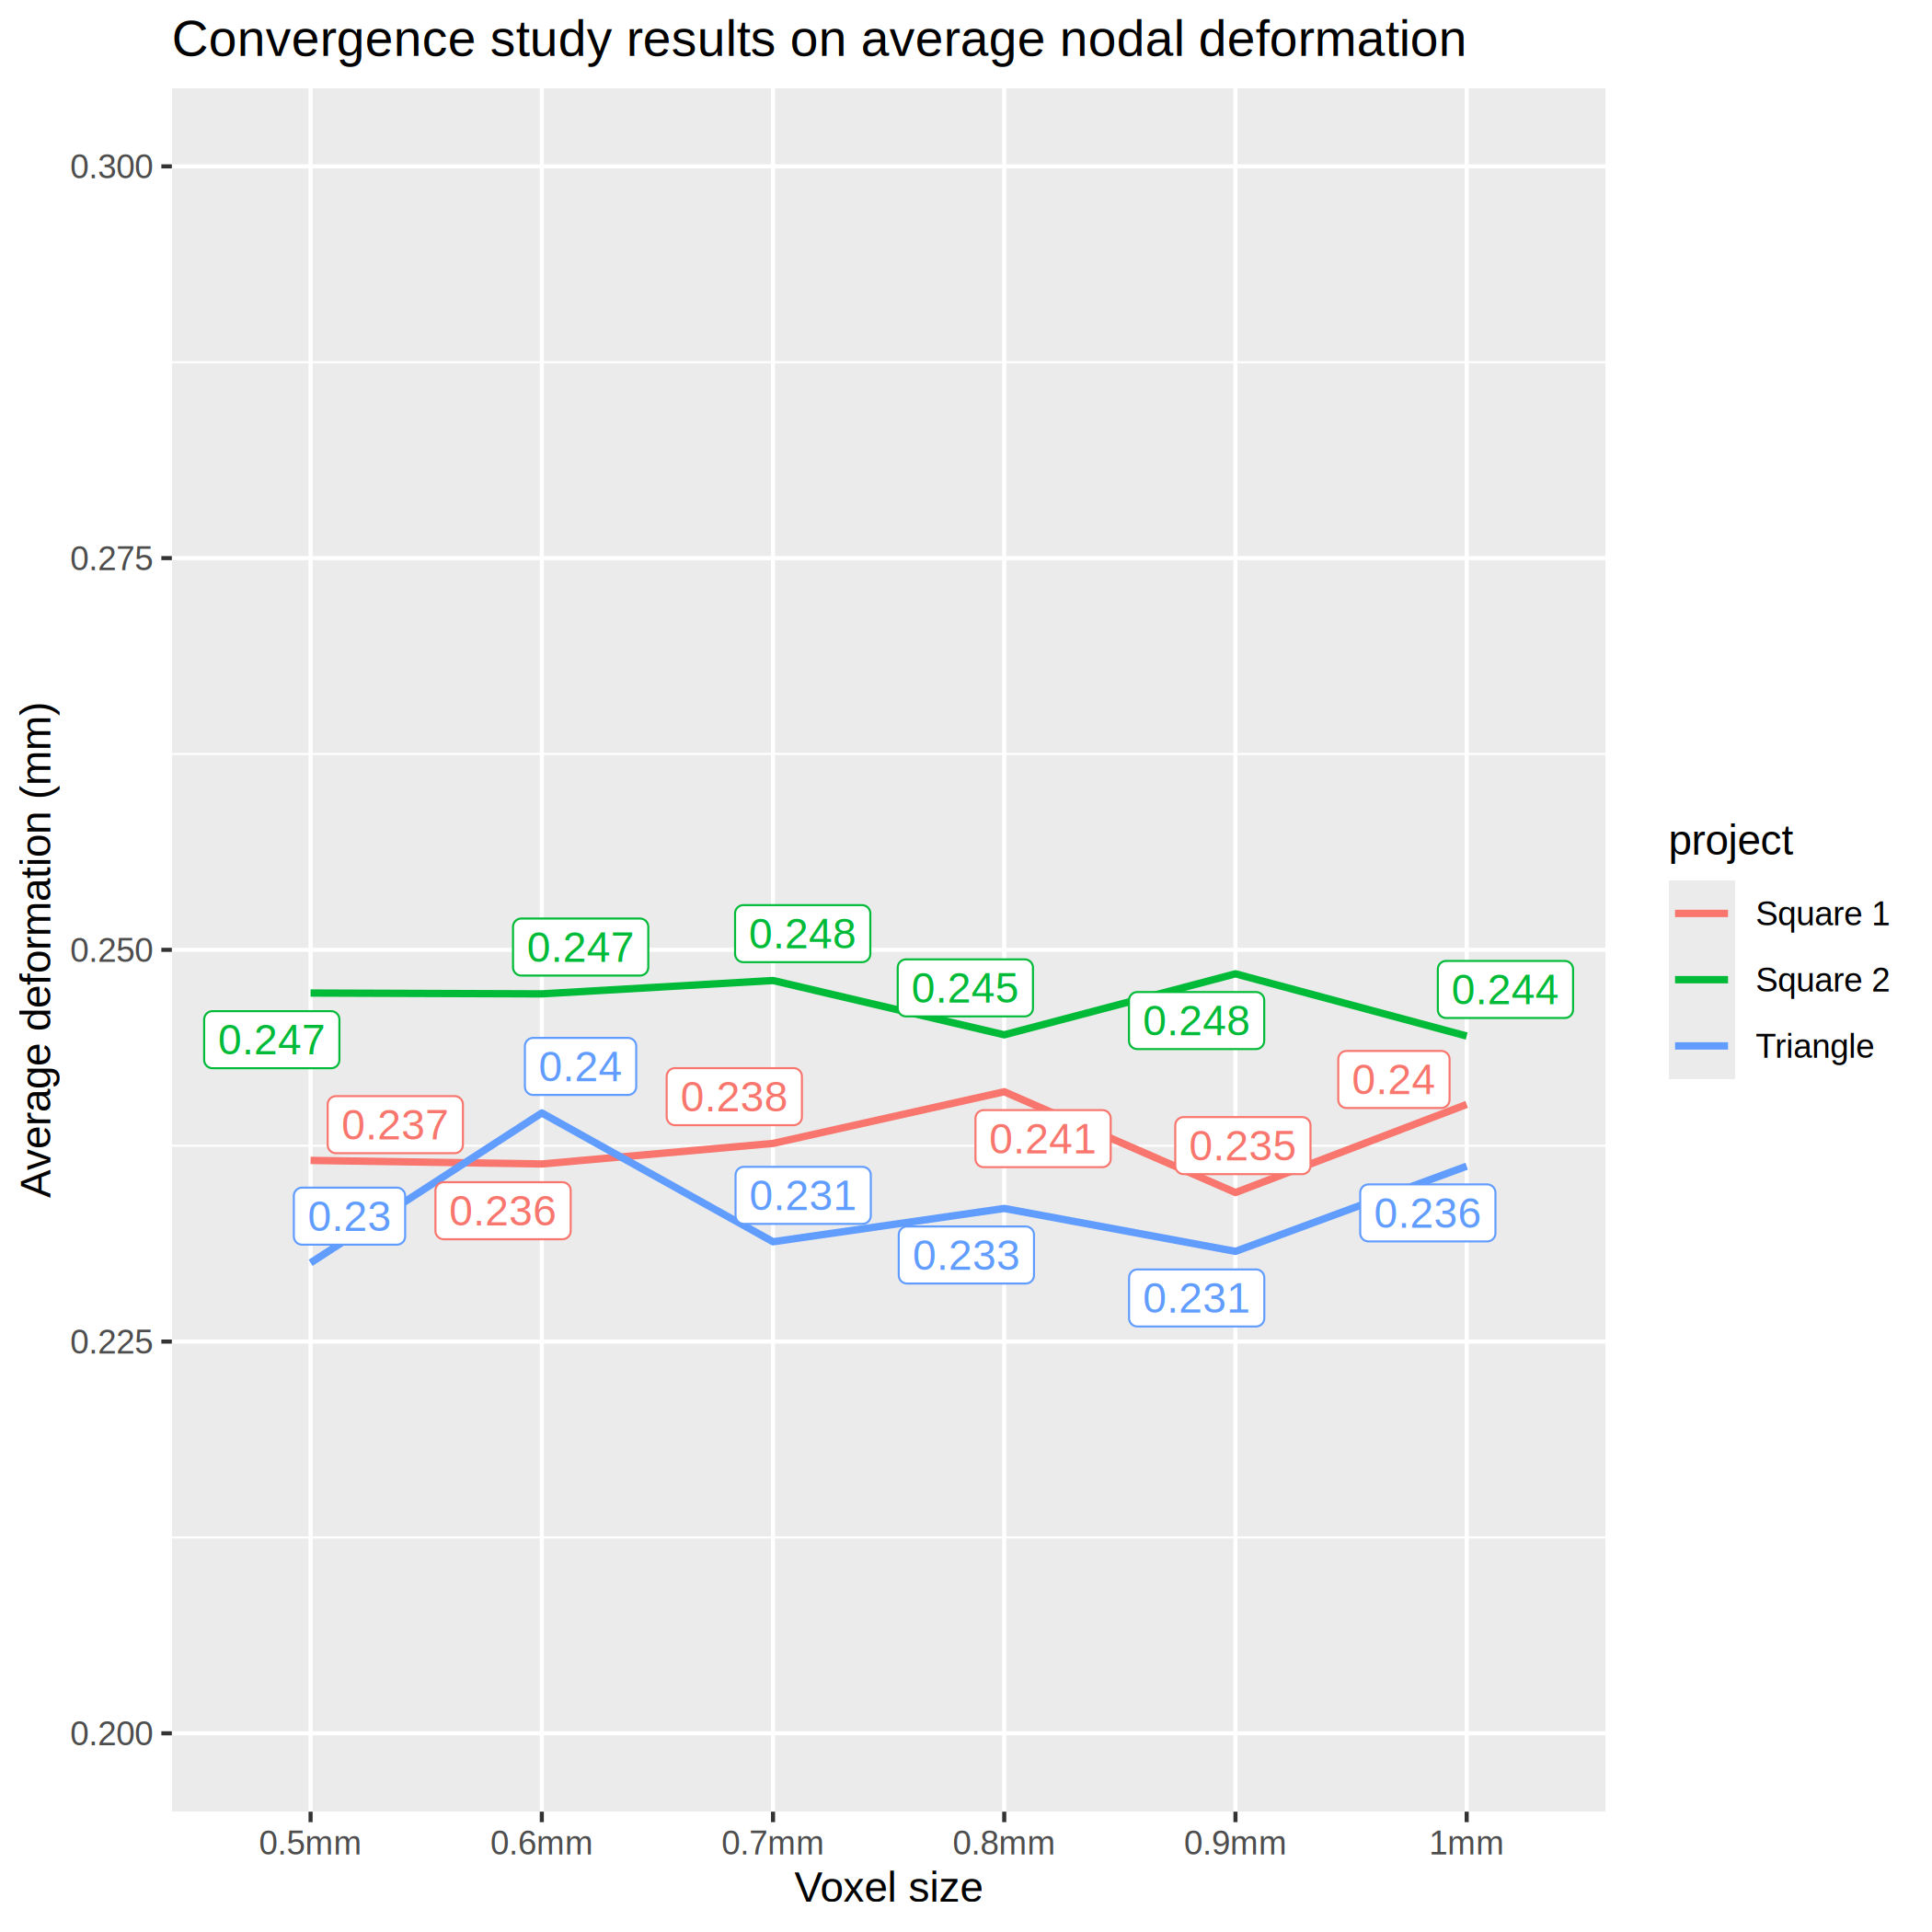
\includegraphics[width=.50\textwidth]{conv_average.png} \hfill
  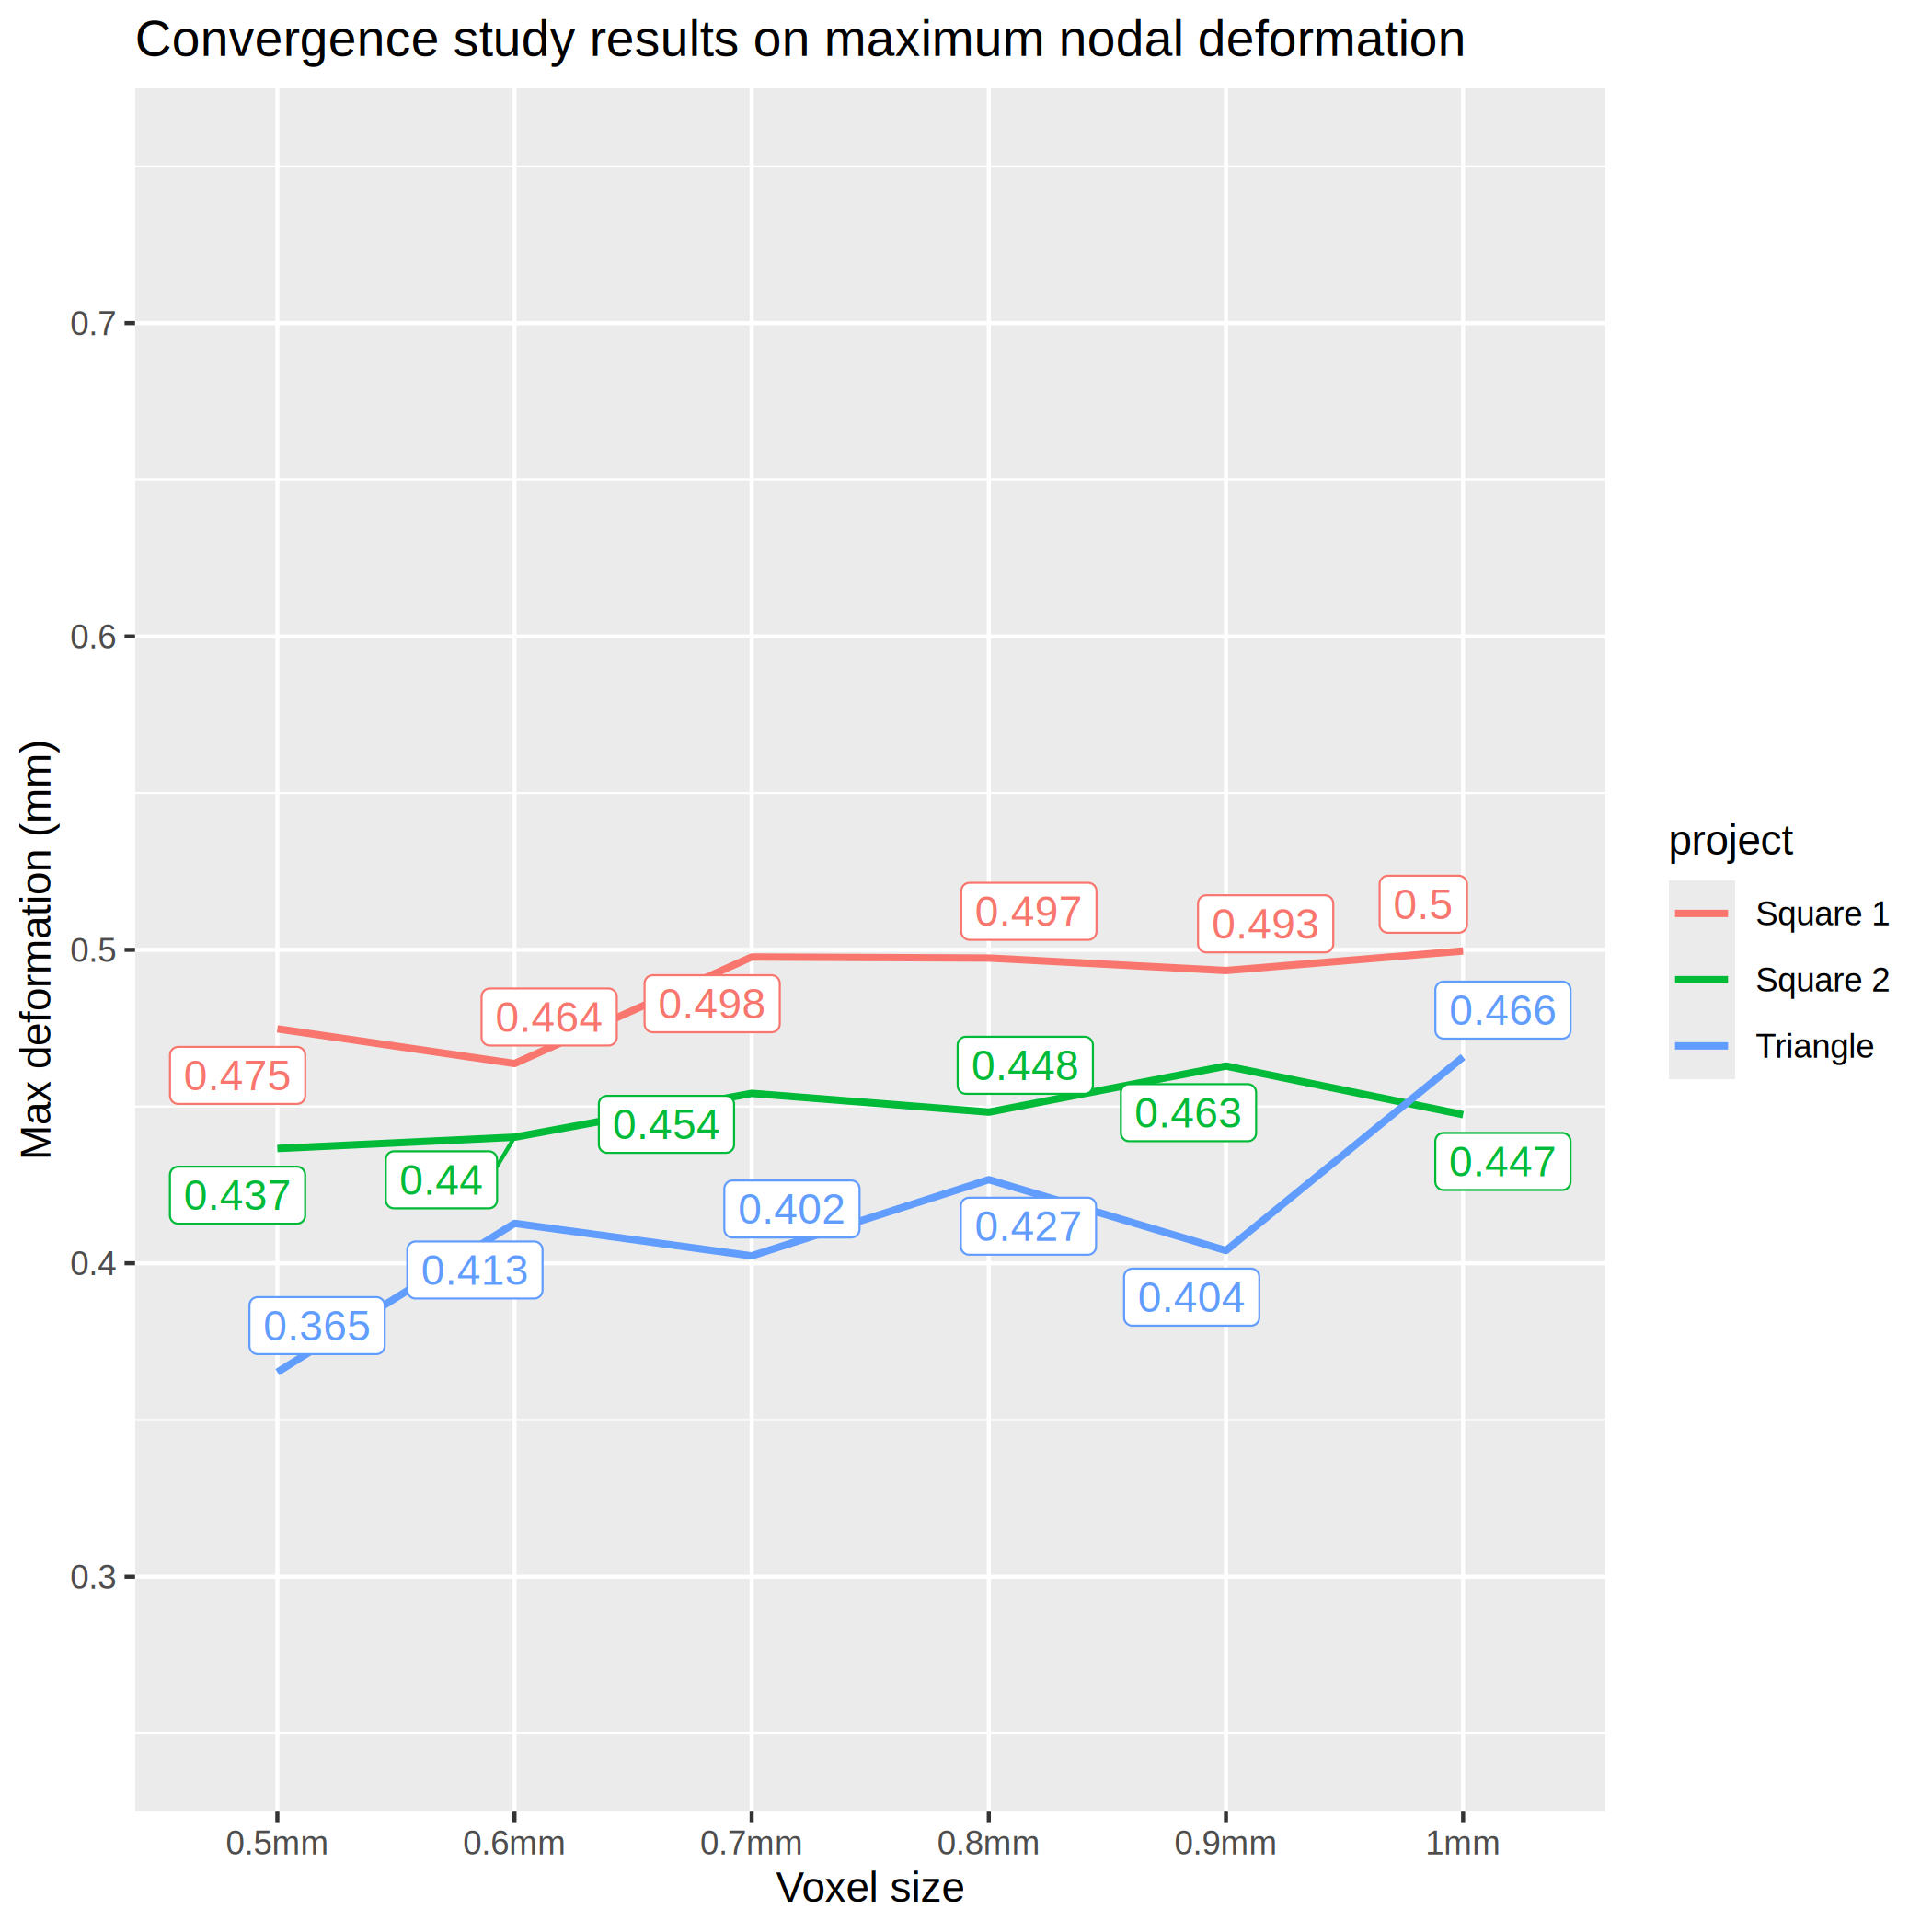
\includegraphics[width=.50\textwidth]{conv_max.png} \hfill
  \caption{Results of convergence test on selected parts.}\label{fig:convergence}

\end{figure}  
\subsection{Voxelization and numerical parameters}

Need to talk about the voxel size and about the solver used

\subsection{Data export}

\textit{This section will detail how I collected the data from Simufact and what software and methods I used to organize it an analyze it. The actual results will go in the following chapter, aptly named results, duh}

\section{Analysis of data}

\todo{Talk about how the data was analyzed, what software and what statistical methods used.}


\listoftodos

\end{document}
